\documentclass[dvipdfmx,uplatex,twocolumn,10pt]{jsarticle}
\usepackage{../sty/macros}

\begin{document}

\begin{figure}[htbp]
\begin{center}
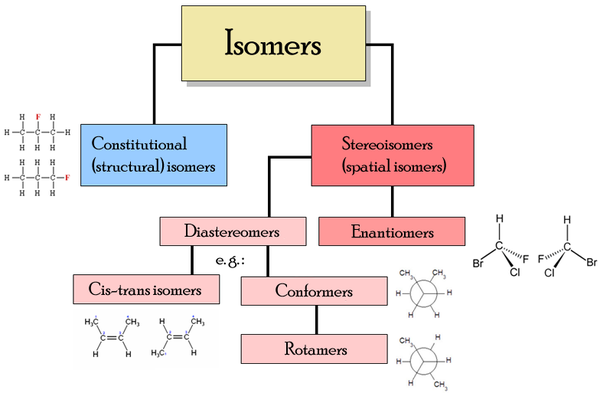
\includegraphics[width=70mm]{600px-Isomerism.png}
\end{center}
\end{figure}

\subsection{構造異性体:structural isomer}
構造異性体(こうぞういせいたい、structural isomer)とは、化学における異性体の分類のひとつで、組成式は等しいが原子の間の結合関係が異なる分子のこと。 \\
すなわち、トポロジカル構造が異なる異性体にあたる。 \\

\subsection{立体異性体:stereoisomer}
立体異性体(りったいいせいたい、stereoisomer)は異性体の一種であり、同じ構造異性体同士で、3次元空間内ではどう移動しても重ね合わせることができない分子をいう。 \\
立体異性が生じる原因には立体配置の違いと立体配座の違いがある。

\subsubsection{立体配置による立体異性体}

立体異性体の種類を表す言葉には歴史的変遷があったが現在の化学における考え方は以下のようなものである。
\begin{itemize}
\item 立体異性体はエナンチオマー(enantiomer)とジアステレオマー(diastereomer)に分かれる
\item ジアステレオマーにはシクロ化合物のシス-トランス異性体(cis-trans isomer)も含む
\item ジアステレオマーには二重結合のシス-トランス異性体も含む
\item 光学異性体(optical isomer)という言葉は推奨しない。
\item 幾何異性体(geometrical isomer)という言葉は推奨しない。
\end{itemize}

\subsubsection{立体異性体/エナンチオマー$\rightarrow$キラリティー}
\begin{defi} \mbox{} \\
キラリティー (chirality) は、3次元の図形や物体や現象が、その鏡像と重ね合わすことができない性質。掌性。 \\
\end{defi}
対掌性(たいしょうせい)ともいう。対掌とは右と左の手のひらの対を意味している。対称性と紛らわしいが、キラリティとは鏡像対称性の欠如であり、むしろ逆の意味になる。 \\
立体図形の対称操作は全て、n回回転 (Cn) と鏡映 (σ) の組み合わせで表せる。 \\
n回回転 (Cn) とはn回の回転で360度回転して元に戻る回転操作で、つまりは360/n度回転させる操作である。従ってC1とは何もしない操作でもある。 \\
n回回転 (Cn )と、その軸に垂直な面での鏡映 (σ) を続けて行う操作をn回回映 (Sn) という。従って1回回映 (S1) とは鏡映に他ならない。一点を中心に図形の全ての点を反対側に映す操作を反転といい i で表すが、これは2回回映 (S2) に等しい。

このような対称操作とキラリティーの関係は表のようにまとめられる。キラルとはSn軸を持たないことと同義である。 \\
鏡映面や反転中心をもたないことは、キラルであることの必要条件であるが十分条件ではない。あくまでも、回映軸が存在するか否かがキラリティーの有無の必要十分条件である。 \\
また、キラル図形は全く対称性を持たないもの(無対称)とnが2以上のCn軸だけ持つものに分類できる。 \\

\begin{defi} \mbox{} \\
キラル中心(キラルちゅうしん、英語: Stereocenter)とは、分子のキラリティーを生じさせる元となる原子をいう[1]。不斉原子または不斉中心ともいう。 \\
\end{defi}
不斉炭素原子は分子がキラルとなるひとつの要因だが、必要条件でも十分条件でもない。アレン誘導体のように、不斉炭素原子を持たないがキラルな分子もある。 \\

\begin{defi} \mbox{} \\
キラルな分子をキラル分子という。 \\
キラル分子は、ちょうど右手と左手のように互いに鏡像である1対の立体異性体を持ち、
これら2つの異性体は互いにエナンチオマー (enantiomer)、対掌体(たいしょうたい。対称体は誤り)、あるいは鏡像異性体(きょうぞういせいたい)であるという。 \\
\end{defi}

キラル分子のエナンチオマーは物質量、結合のエネルギーは等しい。 \\
そのためにほとんどの物理的性質(密度、融点、沸点、屈折率、熱伝導度など)は全く同じである。しかし、旋光性と、ある条件下での化学的性質(生化学的性質を含む)が異なることがある。 \\

\begin{defi} \mbox{} \\
メソ化合物もしくは メソ体 とは立体化学の用語のひとつで、分子内にキラル中心を持つが、同時に対称面も持つためにキラリティーを示さない化合物のこと。メソ(mesos)はギリシャ語で真中を表す。 \\
\end{defi}

\begin{defi} \mbox{} \\
ラセミ体(—たい) (racemate) とは、立体化学の用語で、キラル化合物の2種類の鏡像異性体(エナンチオマー)が等量存在することにより旋光性を示さなくなった状態の化合物のこと。日本語の「ラセミ体」は、ラセミ混合物 (racemic mixture) を表す場合と、ラセミ化合物 (racemic compound) を表す場合とがある。 \\
\end{defi}

キラル化合物の2つのエナンチオマーをそれぞれR体およびS体とすると、ラセミ混合物とはR体とS体とを等モル量混合したもののことであり、ラセミ化合物とはR体とS体の分子が、分子間力や水素結合などの分子間相互作用により 1:1、あるいは n:n の数比でつくった会合体のことである。ラセミ体では各分子の旋光性が互いに打ち消し合い、観測されなくなる。 \\

\subsubsection{立体異性体/ジアステレオマー}
\begin{defi} \mbox{} \\
ジアステレオマー (Diastereomer) は化学物質の異性体のひとつ。立体異性体のうち、鏡像異性体(エナンチオマー)でないものをいう。 \\
\end{defi}
幾何異性体(シス-トランス異性体)もジアステレオマーに含まれる。偏左右異性体という訳語が稀に用いられる。 \\
化合物 A が化合物 B のジアステレオマーである場合、A と B の分子式や化学結合の様式は等しいが、
平行移動や回転操作を施してもぴったりと重ね合わせることはできない。また、A の鏡像も B とは重ならない。 \\
一般に、複数のキラル中心がある化合物はジアステレオマーを持つ。 \\
エナンチオマー同士は旋光性以外の物理的性質が等しいため、キラルカラムを用いたクロマトグラフィーや、酵素や不斉触媒を用いた化学反応など、元々キラリティーを有する物質を作用させる手法でなければ分離することができない。 \\
一方、ジアステレオマー同士は沸点・溶解度・極性などが互いに異なるため、蒸留や再結晶など、キラリティーのない(アキラルな)方法でも分離が可能である。 \\
この性質を利用して、アミノ酸や糖の誘導体など天然から容易に得られるキラル化合物を分離したいラセミ体に結合させ、ジアステレオマーとしてから分離する光学分割が広く行われている。 \\


\subsubsection{立体配座による立体異性体}

液相や気相では、単結合周りの回転は通常は自由であり、多数の異なる形態(立体配座)を取り得る。 \\
従ってこれらの立体配座のいずれかが一致する分子は同じ立体異性体である。 \\
しかし、大きな立体障害などの原因で単結合周りの回転障壁が大きくなると、異なる立体配座を持つ分子同士を分離することができるようになる。 \\
こうして分離された分子同士は、互いに配座異性体(atropisomer /conformer)または回転異性体(rotamer /rotational isomer)であるという。典型的な例はオルト置換ビフェニル誘導体である。 \\

一般的ではないが、二重結合のシス-トランス異性体は非常に回転障壁の高い配座異性体であるという見方もある \\

\subsubsection{用語の変遷}
歴史的には最初、互いに大きさが等しく正負が逆の「旋光性」(光学活性)を示す一対の化合物を互いに「光学異性体」と定義した。 \\
そして旋光性の原因が分子のキラリティーによることが判明すると、「鏡像異性体」、「対掌体」、または「エナンチオマー」の同義語として使われるようになった。 \\
厳密に言えば「光学異性体」は光学活性という観測可能な物性に由来する用語であり、構造に由来する用語である「エナンチオマー」とは別の定義なのだが、実際上はほとんど区別せずに使われてきた。 
また不斉炭素原子を複数持つ分子の異性体である「ジアステレオマー」の概念が登場すると、エナンチオマーとジアステレオマーとを合わせて「光学異性体」とする使い方もなされるようになった。 \\
だが今でも「光学異性体」を「エナンチオマー」の同義語として使っているテキストの方が多い。日本の高校の化学では未だに「光学異性体」という用語を使っているが、高校課程ではジアステレオマーがまだ扱われないため、このような曖昧性はあまり問題にはならないようである。 \\

光学異性 (optical isomerism) という言葉は結晶構造に由来する旋光性に関して使われることもある。これは結晶格子の配置に由来する旋光性であり、特に「左右像 (enantiomorph)」と表される。
\end{document}
